\refstepcounter{section}
\section*{Lecture 1: Introduction and Van der Waal's Equation of State}
\addcontentsline{toc}{section}{Lecture 1: Intro and Van der Waal's Equation of State}
What we will discuss here in mainly the equilibrium physics of phase transitions which is both interesting and intriguing. Phase transitions are generally the result of the collective behaviour of interacting particles which produce some change in the thermodynamics of the system. For interaction between particles, we require a \textit{pair potential}, which describes the behaviour of the interaction. One of such potentials is the celebrated \textit{Lennard-Jones} potential (LJP) which goes as:
$$u(r) = \varepsilon\tund{0}\qty[\qty(\frac{\sigma}{r})^{12}-\qty(\frac{\sigma}{r})^6]$$
where $r = \abs{\vb{r}_i-\vb{r}_j}$ is the interparticle distance. This is used as a model for intermolecular interactions in many systems. Another ``lesser'' realistic (but simpler to handle) model can be described by the potential,
$$u(r) = \begin{cases}
    \infty & r<r\tund{0}\\
    -\varepsilon\tund{0}\qty(\frac{r\tund{0}}{r})^6 & r>r\tund{0}
\end{cases}$$
The above potential tells that the minimum possible separation between molecules is $r\tund{0}$, since $u(r)$ blows up below $r=r\tund{0}$. Hence the particles act as \textit{hard spheres} (spheres which cannot penetrate each other) of radius $\frac{r\tund{0}}{2}$. For $r>r\tund{0}$, $u(r)\sim r^{-6}$ which implies \textit{dipolar interactions}.
\begin{figure}[H]
    \centering 
    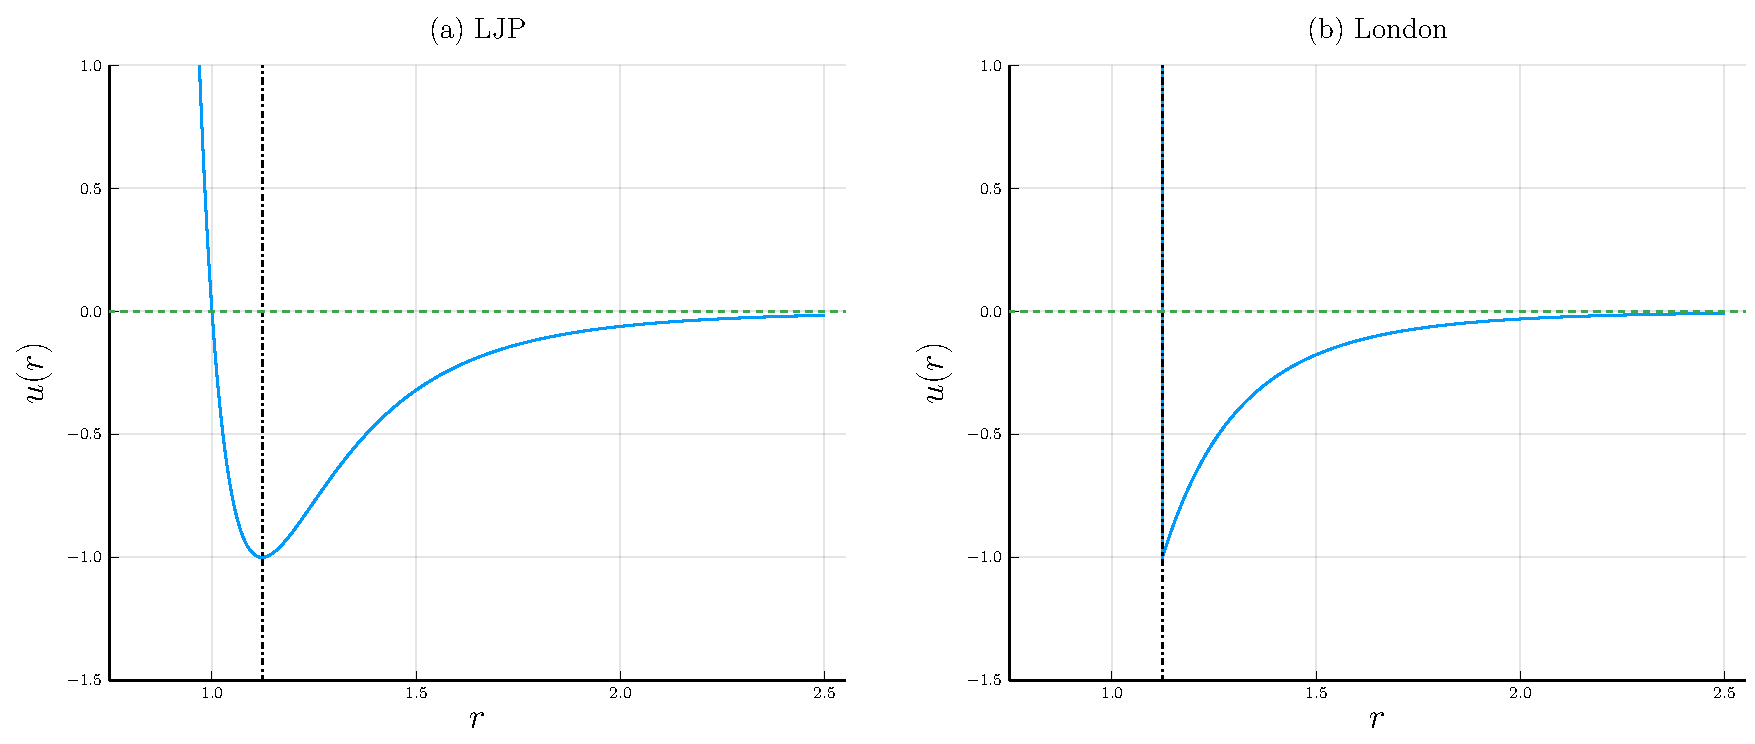
\includegraphics[width=\textwidth]{pics/interactions.pdf}
    \caption{\textbf{Interaction potentials.} (a) Lennard-Jones potential. The vertical line denotes the $r$ at which minima occurs (b) London dispersion potential. }
\end{figure}
\noindent
Note that these interactions are mostly \textit{power-law} interactions, $u(r)\sim r^{-s}$. Let $d$ be the dimension of the space in which we are working. Then, it can be shown or motivated that if $s\leq d$, then the interaction is long-ranged which is not ideal for us. Extensivity can break down and some other issues (like negative specific heat) may occur in this case. One such example is that of gravitational systems where $u(r)\sim \frac{1}{r}$. If $s>d$ then the interaction is short-ranged. Since $u(r)$ blows up when $r=0$, in general, it is advisable to impose a hard core repulsion (like in the London force) which ensures that everything stays okay, since interactions act only after $r>r\tund{0}$ !  
\subsection{Van der Waal's gas}
Let us see an example of this using the Van der Waal's equation which is a correction to the ideal gas equation $PV = N\kb T$ and successfully explains the condensation process of gases.\\[0.2cm]
We will work in canonical ensemble here. The \textit{canonical partition function} is written as,
$$\mathcal{Z}(N,V,T) = \frac{1}{N!}\int \prod\limits_i \qty(\frac{\dd^3 p_i\ \dd^3 q_i}{h^3}) \ e^{-\beta\mathcal{H}}$$
where $\mathcal{H}$ is the Hamiltonian of the system. The $N!$ factor has been put to include the indistinguishability of the particles and $h^3$ factor has been put to make the phase space volume dimensionless. The Hamiltonian consists, as usual, of a kinetic and a pair potential part. 
$$\mathcal{H} = \sum\limits_i \frac{p_i^2}{2m} + \frac{1}{2}\sum\limits_{i\neq j}u(\abs{\vb{q}_i-\vb{q}_j})$$
The momentum integral can be carried out nicely since this is essentially a Gaussian integral. Using independence of the kinetic terms we get,
\begin{align*}
    \mathcal{Z}\tund{p}= \qty[\int \frac{\dd^3 p}{h^3}\ e^{-\beta p^2/2m}]^N=\qty[\frac{4\pi}{h^3}\int\limits_0^\infty p^2 e^{-\beta p^2/2m}\ \dd p]^N  = \qty[\frac{2\pi m \kb T}{h^2}]^{3N/2}
\end{align*}
Defining the thermal wavelength $\lambda\tund{T} = \sfrac{h}{\sqrt{2\pi m \kb T}}$, we have 
$$\SZ = \frac{1}{N!\lambda\tund{T}^{3N}}\int \prod\limits_i \dd^3 q_i\ e^{-\beta U(\{\vb{q}_i\})}$$
where $U(\{\vb{q}_i\})$ denotes the interaction term in the Hamiltonian. Tackling this part is extremely hard, since the interactions are between pair of particles, hence independence cannot be assumed.

\subsection{Uniform Density Approximation}
One of the most popular ways to deal with interactions is through \textit{perturbation}, however, perturbations are generally taken to be \textit{continuous} and hence, non-analyticity (an important aspect of phase transitions) cannot be effectively captured. We will use the method of \textit{mean-field approximation}, which treats the interactions as an ``effective potential'' which can be found out self-consistently. To simplify our calculations, let us define the number density of the gas, in terms of the delta function, 
$$n(\vb{q}) = \sum\limits_{i=1}^N\ \delta^{(3)}(\vb{q}-\vb{q}_i)$$
Then the interaction term becomes,
\begin{align*}
   2U &=\sum\limits_i\sum\limits_{j\neq i} u(\abs{\vb{q}_i-\vb{q}_j})\\
   &=\sum\limits_i\sum\limits_{j\neq i} \int\dd q_1\ \delta^{(3)}(\vb{q}_1-\vb{q}_i)\cdot u(\abs{\vb{q}_1-\vb{q}_j})\\
   &=\sum\limits_i\sum\limits_{j\neq i} \int\dd q_1\ \delta^{(3)}(\vb{q}_1-\vb{q}_i)\cdot \int\dd q_2 \ \delta^{(3)}(\vb{q}_2-\vb{q}_j)\cdot u(\abs{\vb{q}_1-\vb{q}_2})\\
   &=\int\dd q_1\dd q_2\ \sum\limits_i\sum\limits_{j\neq i} \delta^{(3)}(\vb{q}_1-\vb{q}_i)\cdot  \ \delta^{(3)}(\vb{q}_2-\vb{q}_j)\cdot u(\abs{\vb{q}_1-\vb{q}_2})\\
   &=\int\dd q_1\dd q_2\ n(\vb{q}_1)n(\vb{q}_2)u(\abs{\vb{q}_1-\vb{q}_2})
\end{align*}
We will use a heavily \textit{unmotivated} approximation where we will treat the density to be uniform, independent of the spatial coordinate, that is, $n(\vb{r})\equiv n$
Then, 
$$U = \frac{n^2}{2}\int\dd q_1^3 \dd q_2^3\ u(\abs{\vb{q}_1-\vb{q}_2})$$
Let us define the variables $\vb{R} = \frac{1}{2}(\vb{r}_1+\vb{r}_2)$ and $\vb{r} = \vb{r}_1-\vb{r}_2$ from which we have $\vb{r}_1 = \vb{R}+\frac{\vb{r}}{2}$ and $\vb{r}_2 = \vb{R}-\frac{\vb{r}}{2}$. The Jacobian of this transformation can be written as,
$$\mathrm{\vb{J}} \equiv \pdv{(\vb{r}_1, \vb{r}_2)}{\vb{R}, \vb{r}} =\mqty(\iden & \frac{1}{2}\iden\\ \iden & -\frac{1}{2}\iden) \implies J = \det({\mathrm{\vb{J}}}) = -1$$
Using the new variables, the integral becomes, 
$$U = \frac{n^2}{2}\int \dd^3 R\ \dd^3 r \ u(r) = \frac{n^2V}{2}\int\limits_{r\tund{0}}^\infty \dd^3 r \ u(r)= \frac{N^2}{2V}\int \dd^3 r \ u(r)$$
where we have used $n = \sfrac{N}{V}$ and $r\tund{0}$ is the hard-core cutoff. Now, assume a power-law interaction for $r>r\tund{0}$, 
$u(r) = -\varepsilon\tund{0}\qty(\frac{r\tund{0}}{r})^s$ using which we get, 
\begin{align*}
    U =-\frac{\varepsilon\tund{0} N^2}{2V}\cdot r\tund{0}^s \int\limits_{r\tund{0}}^\infty 4\pi r^2 \dd r\ \frac{1}{r^s} = -\frac{4\pi\varepsilon\tund{0} N^2r\tund{0}^s}{2V(3-s)}\ r^{3-s}\Bigg|^\infty_{r\tund{0}}
\end{align*}
As we can see, $U$ is finite only when $3-s<0\implies s>3$ where $3$ was our spatial dimension. Assuming $s>3$, we have $r^{3-s}\to 0$ and we have 
$$U = \frac{4\pi\varepsilon\tund{0} N^2r\tund{0}^s}{2V(3-s)}r\tund{0}^{3-s} = -\frac{4\pi\varepsilon\tund{0} N^2r\tund{0}^3}{2V(s-3)} = -\frac{aN^2}{V}\qquad \text{where,}\ \  a\equiv \frac{2\pi \varepsilon\tund{0}r\tund{0}^3}{s-3} $$
We get an `effective' interaction potential using the \textit{uniform density approximation}. From here, the partion function now becomes,
$$\SZ = \frac{e^{\beta aN^2/V}}{N! \lambda\tund{T}^{3N}}\int \prod\dd q_i$$
Now, the integral is simply not equal to $V^N$, since we have assumed a hard-sphere gas and each particle has some finite volume. Assume that each particle occupies a small volume $\omega$, which cannot be occupied by the other particles. If one particle occupies volume say $V$, then the second particle can occupy $V-\omega$, the third occupies $V-2\omega$ and so on. Then the integral will be just,
\begin{align*}
    \int \prod \dd q_i \equiv \prod\limits_{i=0}^{N-1} (V-i\omega) &\approx \prod (V-j\omega)(V-(N-j)\omega)\\
&=\prod V^2\qty(1 - \frac{j\omega}{V})\qty(1 - \frac{(N-j)\omega}{V})\\
&\approx V^N \prod \qty[1 - \frac{(j+N-j)\omega}{V}+ \SO(\qty(\sfrac{\omega}{V})^2)]\\
&\approx V^N\qty[1 - \frac{N\omega}{V}]^{N/2} = \qty[V\qty(1-\frac{N\omega}{V})^{1/2}]^N
\end{align*}
where we have made the product over $\approx N/2$ pairs. Now, assume $N\omega \ll V$ from which we can use the approximation $(1+x)^n \approx 1+nx$ to get,
$$\qty[V\qty(1-\frac{N\omega}{V})^{1/2}]^N \approx \qty[V\qty(1-\frac{N\omega}{2V})]^N = \qty[V-\frac{N\omega}{2}]^N$$
We see that the available volume is reduced by a factor of $N\omega/2$. This was the final step and we can now write the partition function,
$$\boxed{\SZ(N,V,T) = \frac{e^{\beta aN^2/V}}{N! \lambda\tund{T}^{3N}}\qty[V-\frac{N\omega}{2}]^N }$$
The free energy can be obtained from the partition function using $F = -\kb T \ln \SZ$,
$$F = -\cancel{\kb T} \cancel{\beta} \frac{a N^2}{V}-N\kb T \ln\qty[V-\frac{N\omega}{2}]+c(N,T)$$
and from here, we can find the pressure $P = - \qty(\pdv{F}{V})_{N,T}$ 
\begin{align*}
    P &=-\frac{aN^2}{V^2} +\frac{N\kb T}{\qty(V-\frac{N\omega}{2})} \implies \boxed{\qty(P+\frac{aN^2}{V^2})\qty(V-Nb) = N\kb T}
\end{align*}
This is the Van der Waal's equation, where we have defined $b = \sfrac{\omega}{2}$. This can be written in an alternate form using the number of moles, $\mathfrak{n} = \sfrac{N}{N\tund{A}}$ where $N\tund{A}$ is the Avogadro's number:
$$\qty(P+\frac{a'\mathfrak{n}^2}{V^2})\qty(V-\mathfrak{n}b') = \mathfrak{n}RT\iff \qty(P+\frac{a'}{v_m^2})\qty(v_m-b') = RT$$
where $a' = N\tund{A}^2 a$ and $b' = b N\tund{A}$ and $v_m$ is the molar volume. 

